% =========================================================================
% Section 5 — Results
% Fragment for \input from main.tex (no preamble).
% =========================================================================
\section{결과}
\label{sec:results}

본 절에서는 DefectSegAM 의 평가를 네 부분으로 나누어 보고한다. 앞의 세
부분은 완료된 측정을 보고한다. 즉, ORNL 빌드에서 DefectSegAM 과
production DSCNN 간의 일치도(agreement)
분석(\ref{sec:results-agreement}절), 다운스트림 인장 물성 사례
연구(\ref{sec:results-downstream}절), 그리고 계산 효율
프로파일(\ref{sec:results-efficiency}절; 파라미터 수와 학습 메모리는
보고하며 추론 시간 측정은 미완료)이다. 마지막
부분(\ref{sec:results-planned}절)은 \ref{sec:setup}절에서 정의한
프로토콜을 따르지만 아직 수행되지 않은 세 가지 평가---사람이 주석한
ground truth 상에서 재구현 DSCNN 과 비교하는 held-out 평가, cross-machine
일반화 연구, 그리고 구성 요소 ablation---를 한데 묶어 실험
스캐폴드(scaffold)로 제시한다.

% -------------------------------------------------------------------------
\subsection{ORNL 빌드에서 production DSCNN 과의 일치도}
\label{sec:results-agreement}

본 소절의 모든 정량 수치는 Stage-1 의사 라벨(pseudo-label) teacher 로
쓰인 production DSCNN~\cite{Scime2020DSCNN}의 세그멘테이션 맵---ORNL
Co-Registered 데이터셋~\cite{ORNL_CoRegistered_Dataset}에서 빌드 규모로
이용 가능한 유일한 참조 라벨---에 대한 \emph{일치도(agreement)} 통계로서,
student 가 teacher 로부터 얼마나 벗어나는지를 보이기 위해 보고하는
것이지 정확도가 아니다(\ref{sec:setup-metrics}절). 추론 설정은
\ref{sec:setup-impl}절의 기본값(단일 forward pass)을 따른다.

\paragraph{검증 빌드에서의 학습 시점 일치도}
고정 검증 빌드 B1.1 에서, Stage-1(의사 라벨 사전학습) best checkpoint 는
전체 3{,}218-레이어 검증 세트에 대해 production DSCNN 과 0.9738 의 픽셀
수준 일치도와 0.2573 의 11-class mIoU 에 도달하였다. 전문가 주석에 대한
Stage-2 미세조정 이후, best checkpoint 는 모델 선택에 사용한 200-레이어
평가 부분집합에서 0.9756 의 픽셀 일치도와 0.2952 의 mIoU 에 도달하였다.
전체 3{,}218-레이어 검증 빌드에서 평가하면, Stage-2 의 per-class IoU 값은
0.9744 (Powder), 0.9137 (Printed), 0.1252 (Recoater Streaking), 0.3106
(Swelling; precision 0.5211, recall 0.4347), 0.3271 (Spatter; recall
0.9929)이다. 이러한 낮은 결함 클래스 값은 주의 깊게 해석해야 한다. 빌드
B1.1 은 정상(nominal) 공정 조건에서 프린트되었고 11개 클래스 중
4개(Recoater Hopping, Debris, Over Melting, Under Melting;
Super-Elevation 의 support 는 2 픽셀뿐)에 대해 참조 픽셀이 사실상
전무하므로, B1.1 에서의 일치도로는 해당 클래스를 전혀 평가할 수 없다.
Recoater Streaking 과 Spatter 의 recall 우세 프로파일(Stage-1 recall 이
각각 0.8707 과 0.9941, precision 은 각각 0.1253 과 0.3094)은 DefectSegAM
이 이들 결함을 production 모델보다 더 넓은 영역에 라벨링함을 나타낸다.
이는 teacher 대비 체계적인 과탐지(over-detection)로, 그 결과는 아래에서
정성적으로, 그리고 \ref{sec:results-downstream}절에서 정량적으로 검토한다.

\paragraph{다중 빌드 일치도 및 이전 모델 세대와의 비교}
표~\ref{tab:results-agreement-miou}는 세 개 빌드(B1.1, B1.2, B1.5)
각각에서 균일하게 샘플링한 150개 레이어에 대한 최종 Stage-2 모델의 일치도
mIoU 를 보고한다. 이때 데이터셋 제공 12-class 맵을 표~\ref{tab:classes}의
11-class 공간으로 재매핑하고(Misprint 무시), support 가 0이 아닌 클래스들에
대해 평균을 취하였다. 맥락 제공을 위해 두 개의 이전 내부 모델 세대를
포함하였다: v1(ViT-S/14 백본, native 12-class head)과 v3(ViT-S/14, Under
Melting 클래스가 없는 10-class head). 정상 조건 빌드 B1.1 과 손상 리코터
빌드 B1.5 에서는 세 세대 모두 production 모델과 유사한 정도로
일치한다(mIoU 0.43--0.52). 차이는 의도적인 lack-of-fusion 및 keyhole
조건을 포함한 네 가지 파라미터 세트로 프린트된 결함 다수(defect-rich)
빌드 B1.2 에서 나타난다. 여기서 DefectSegAM 은 0.5047 의 일치도 mIoU 에
도달한 반면, v1 은 0.4455, v3 은 0.4291 이었다.

\begin{table}[t]
\centering
\caption{각 모델 세대와 production DSCNN 간의 일치도 mIoU(DSCNN 일치도;
\ref{sec:setup-metrics}절). ORNL 빌드별로 균일하게 샘플링한 150개
레이어에 대해 산출하였다(참조 맵: 데이터셋 제공 12-class 세그멘테이션을
11 클래스로 재매핑, Misprint 무시; support 가 0이 아닌 클래스들에 대한
평균).}
\label{tab:results-agreement-miou}
\footnotesize
\begin{tabular}{lccc}
\toprule
빌드 & \makecell{v1\\(ViT-S, 12-class)} & \makecell{v3\\(ViT-S, 10-class)} & \makecell{DefectSegAM\\(ViT-B, 11-class)} \\
\midrule
B1.1 (정상 조건)        & 0.4483 & 0.4310 & 0.4362 \\
B1.2 (결함 다수)        & 0.4455 & 0.4291 & \textbf{0.5047} \\
B1.5 (손상 리코터)      & 0.5200 & 0.4880 & 0.4823 \\
\bottomrule
\end{tabular}
\end{table}

표~\ref{tab:results-agreement-perclass}는 B1.2 결과를 클래스별로 분해한
것이다. 이전 세대 대비 DefectSegAM 의 이득은 B1.2 밖에서는 거의 존재하지
않는 두 용융 에너지 클래스가 주도한다. Under Melting 은 0.8643 의 일치도
IoU 에 도달하고(v3 은 Under Melting 클래스가 없어 0.0 이며, v1 은 0.7887),
Over Melting 은 0.4715 에 도달한다(v3: 0.4587; v1: 0.0690). Over Melting
과 Under Melting 은 각각 keyhole 및 lack-of-fusion 기공의 DSCNN 측
전조(precursor)이므로, 이들이 실제로 발생하는 빌드에서 해당 채널을
일관되게 재현하는 것은 \ref{sec:results-downstream}절의 다운스트림 물성
연구를 위한 전제 조건이 된다.

\begin{table}[t]
\centering
\caption{빌드별로 균일하게 샘플링한 150개 레이어에 대한 DefectSegAM(최종
Stage-2 모델)과 production DSCNN 간의 per-class 일치도 IoU.
``---'' 는 샘플링된 레이어에서 참조 support 가 0인 클래스를 표시하며,
이들은 mIoU 에서 제외된다. B1.2 는 희소한 용융 관련 클래스에 유의미한
support 를 제공하는 유일한 빌드이다. B1.2 의 참조 support 는 Swelling
852{,}040 픽셀, Super-Elevation 1{,}396 픽셀이다(150개 레이어 합;
\ref{sec:discussion-taxonomy}절에서 참조).}
\label{tab:results-agreement-perclass}
\footnotesize
\begin{tabular}{lccc}
\toprule
클래스 & B1.1 & B1.2 & B1.5 \\
\midrule
Powder                & 0.9742 & 0.9553 & 0.9401 \\
Printed               & 0.9220 & 0.8395 & 0.9039 \\
Recoater Hopping      & ---    & ---    & ---    \\
Recoater Streaking    & 0.1086 & 0.4830 & 0.3776 \\
Incomplete Spreading  & 0.0000 & 0.1073 & ---    \\
Swelling              & 0.2710 & 0.6038 & 0.2691 \\
Debris                & ---    & 0.0100 & ---    \\
Super-Elevation       & ---    & 0.0043 & ---    \\
Spatter               & 0.3417 & 0.7083 & 0.4031 \\
Over Melting          & ---    & 0.4715 & 0.0000 \\
Under Melting         & ---    & 0.8643 & ---    \\
\midrule
mIoU (support $>$ 0)  & 0.4362 & 0.5047 & 0.4823 \\
\bottomrule
\end{tabular}
\end{table}

\paragraph{정성적 비교}
그림~\ref{fig:qualitative-dscnn}은 다섯 개 ORNL 빌드 전체에서 샘플링한
레이어에 대해 DefectSegAM 라벨 맵과 데이터셋 제공 DSCNN 맵을 비교한
것이다. 위의 recall 우세 일치도 프로파일과 일관되게, DefectSegAM 은 원본
이미지에서 관찰되는 것보다 다소 넓은 결함 영역을 예측하는 경미한
과탐지(over-detection) 경향을 보이지만, production DSCNN 이 부분적으로만
검출하거나 완전히 놓치는 Recoater Streaking 및 Spatter 영역을 일관되게
포착한다. 더 넓은 검출 범위가 오류인지 교정인지는 이 이미지들만으로 판단할
수 없으며, \ref{sec:results-heldout}절의 held-out 사람 GT 평가가 바로 이
질문에 답하도록 설계되어 있다.

\begin{figure}[tp]
\centering
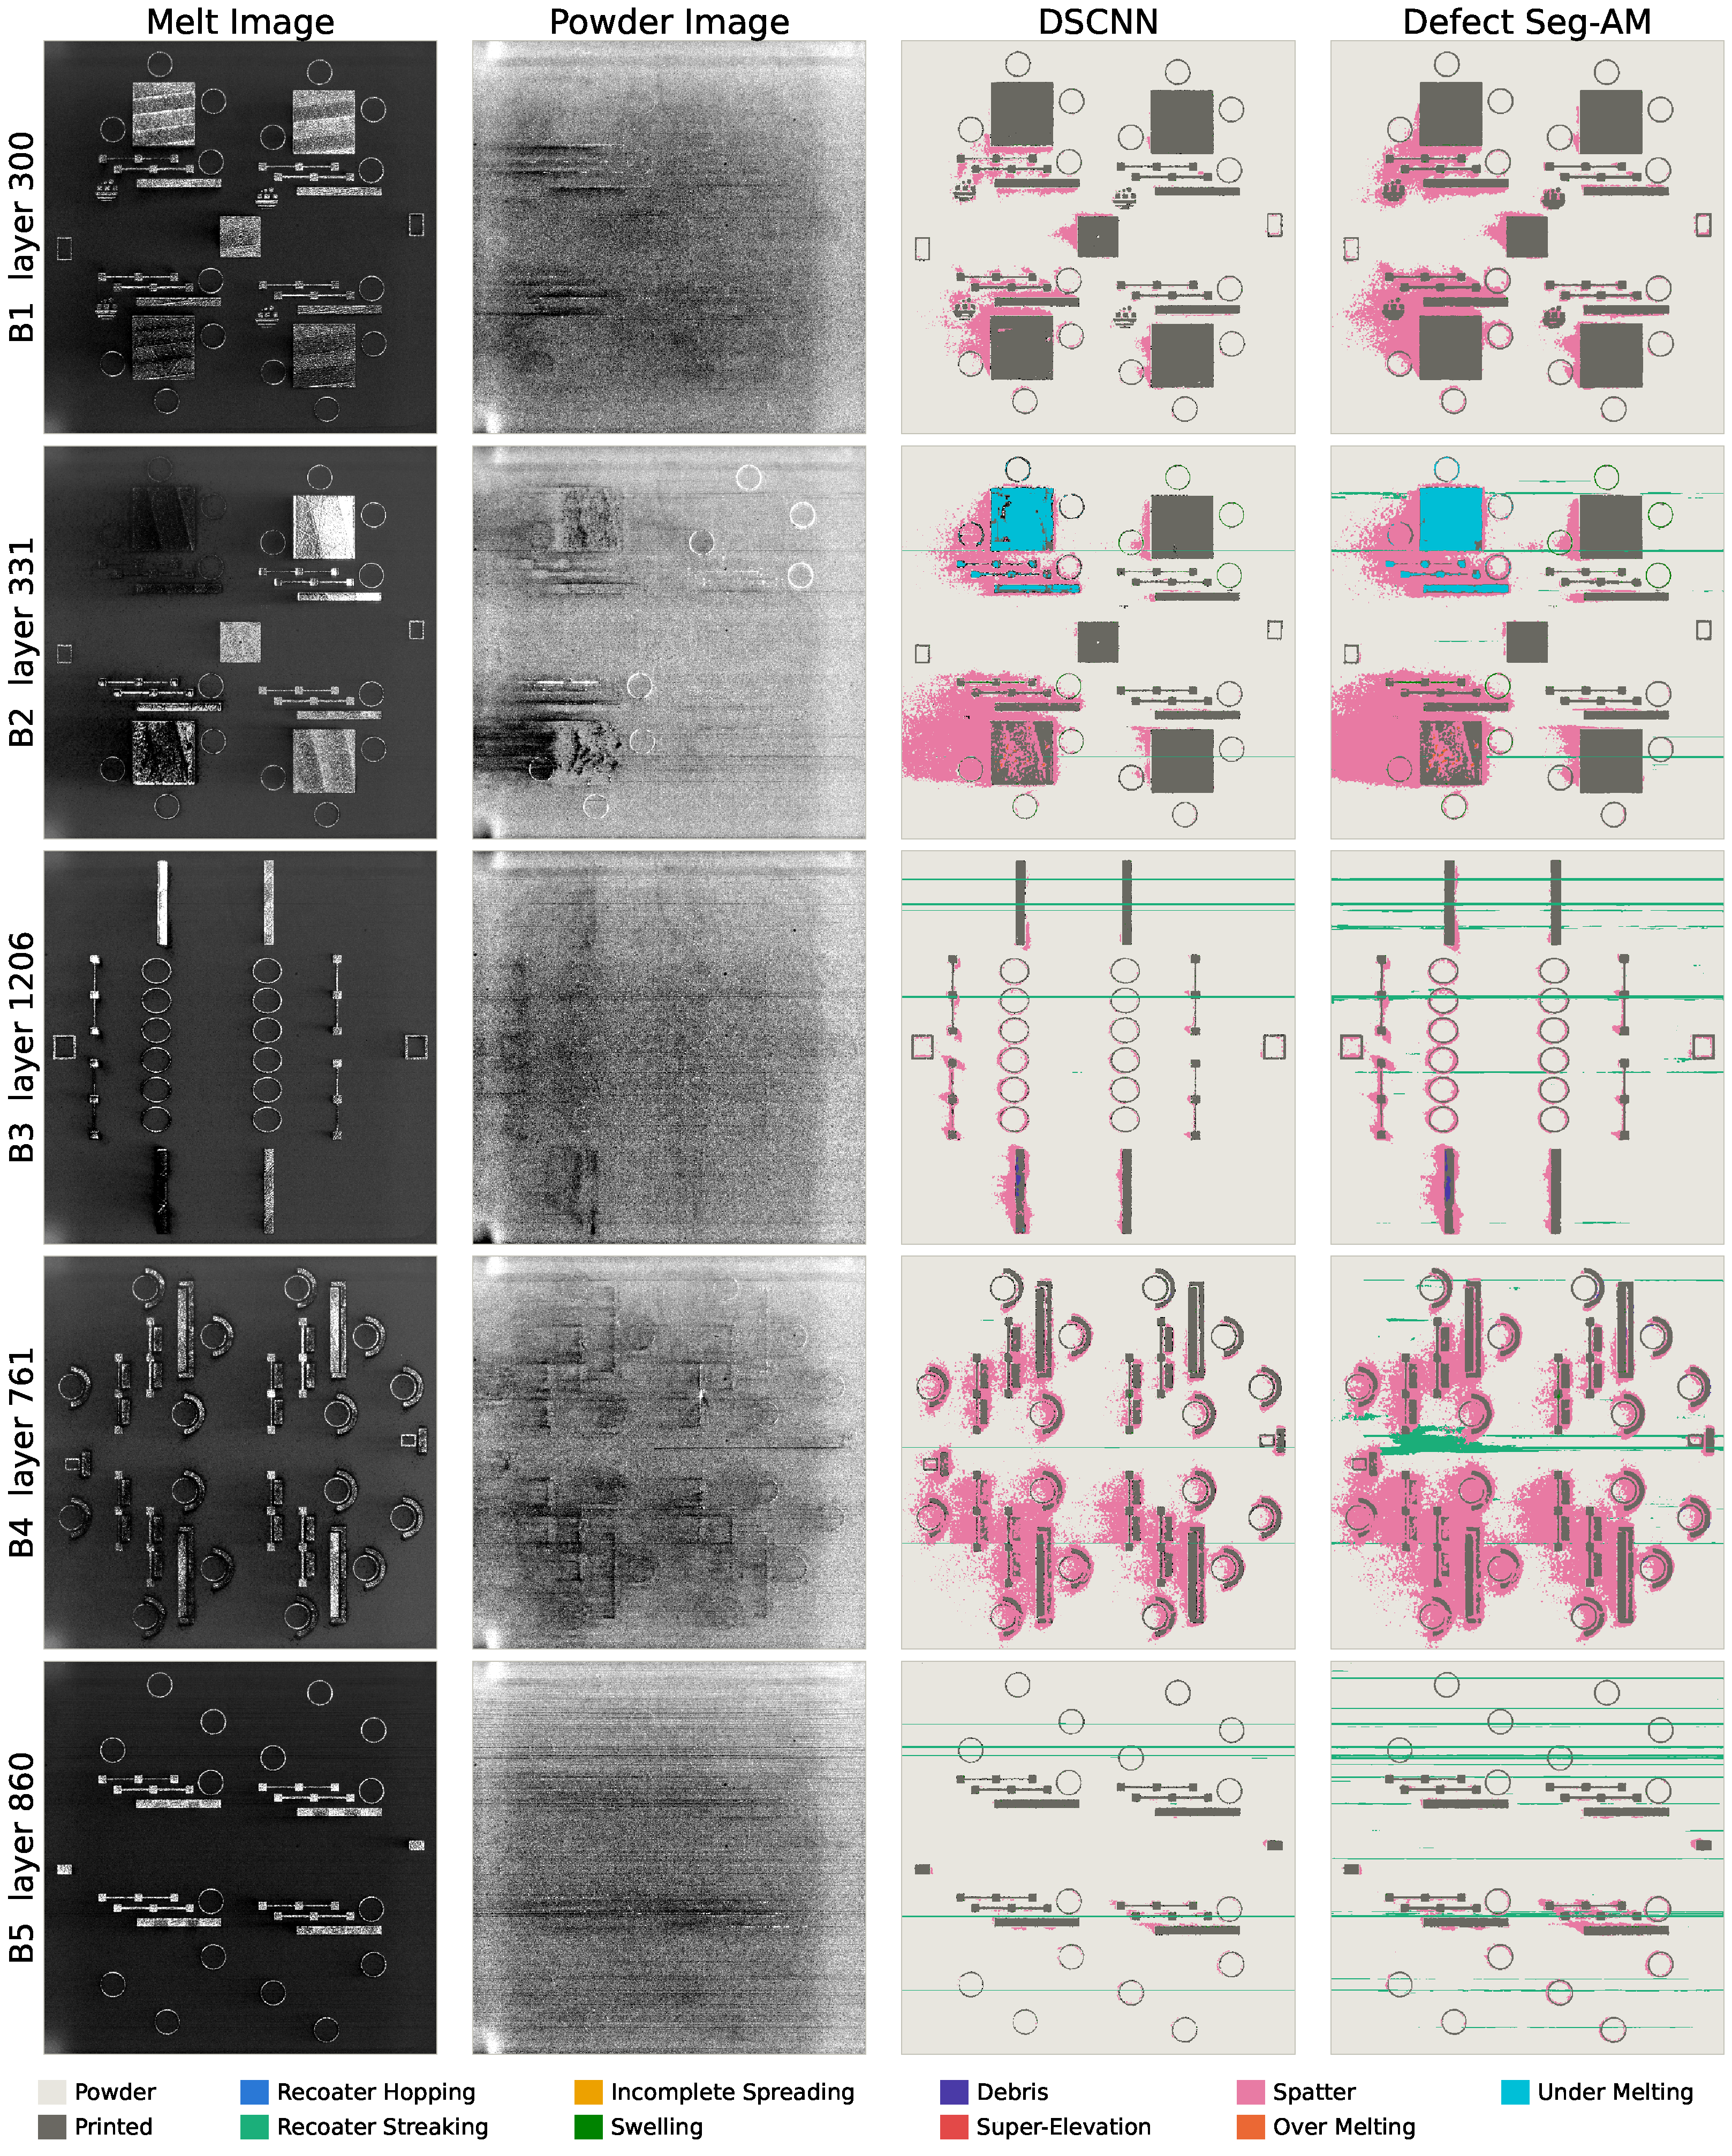
\includegraphics[width=\linewidth,height=0.80\textheight,keepaspectratio]{Figs/Image_Seg_Compare_DSCNN_vs_DefectSegAM.pdf}
\caption{다섯 개 ORNL 빌드 전체에서 샘플링한 대표 레이어에 대한 데이터셋
제공 production DSCNN 세그멘테이션(가운데)과 DefectSegAM(오른쪽)의 정성적
비교. 대응하는 원본 가시광 레이어 이미지를 왼쪽에 함께 나타냈다.
DefectSegAM 은 원본 이미지에서 관찰되는 것보다 다소 넓은 결함 영역을
예측하는 경미한 과탐지 경향을 보이지만, production DSCNN 이 부분적으로만
검출하거나 완전히 놓치는 Recoater Streaking 및 Spatter 영역을 일관되게
포착한다. 두 모델 모두 test-time augmentation 및 후처리 없이 나타냈다.}
\label{fig:qualitative-dscnn}
\end{figure}

% -------------------------------------------------------------------------
\subsection{다운스트림 인장 물성 사례 연구}
\label{sec:results-downstream}

ORNL 빌드에는 held-out 세그멘테이션 ground truth 가 없으므로, 해당
데이터셋에서는 DefectSegAM 과 production DSCNN 간의 직접적인 정확도 비교가
불가능하다. 따라서 본 연구에서는 두 세그멘테이션 소스를 그 출력의
다운스트림 유용성, 즉 그 외 조건이 동일한 인장 물성 예측 파이프라인에 각
소스가 물성 관련 정보를 얼마나 제공하는지를 기준으로 평가한다. 슈퍼복셀
집계, 소스별 채널 집합, 회귀 모델, 시편 단위 5-fold 교차검증 분할과 보고
방식은 모두 \ref{sec:setup-downstream}절의 프로토콜을 따른다.

표~\ref{tab:downstream}과 그림~\ref{fig:downstream}은 그 결과를 요약한다.
데이터셋 제공 DSCNN 맵을 사용하면 segmentation-only 예측기는 붕괴한다.
UTS RMSE $70.7 \pm 2.5$\,MPa 는 naive 전역 평균 예측기의 68.4\,MPa 보다
오히려 \emph{더 나쁘고}(3.4\,\% 악화), YS 역시 1.2\,\% 악화되며, UE 와 TE
는 각각 3.6\,\% 와 5.5\,\% 개선에 그친다. 이 붕괴의 원인은 맵 자체로
추적된다. 데이터셋 제공 세그멘테이션에서 유도한 슈퍼복셀 집계 결함 채널
피처의 평균은 약 0.001--0.008 에 불과하여 회귀기가 활용할 시편 간 분산이
사실상 남지 않으므로, 모델은 전역 평균을 출력하는 것 이상을 거의 할 수
없다. 동일한 DSCNN 채널에 대해 MLP 를 순환(recurrent) 인코더로 교체해도
같은 붕괴가 재현되며(UTS RMSE 64.8\,MPa), 이는 병목이 회귀 아키텍처가
아니라 세그멘테이션 소스임을 확인해 준다.

\begin{table}[t]
\centering
\caption{ORNL 데이터셋에서 \ref{sec:setup-downstream}절의 프로토콜(5-fold
시편 단위 교차검증, $N = 6{,}373$ 시편)로 평가한 segmentation-only VPPM
변형들의 시편 수준 RMSE. 항복강도(YS), 인장강도(UTS), 균일연신율(UE),
총연신율(TE)에 대해 보고한다. 학습되는 두 변형은 세그멘테이션 소스만
다르다. $\pm$ 는 다섯 개 fold 에 걸친 RMSE 의 표준편차를 나타내며,
naive(전역 평균) 예측기는 fold 가 없다.}
\label{tab:downstream}
\footnotesize
\begin{tabular}{lcccc}
\toprule
예측기 & YS (MPa) & UTS (MPa) & UE (\%) & TE (\%) \\
\midrule
Naive (전역 평균)              & 33.9 & 68.4 & 15.0 & 18.5 \\
DSCNN 기반 (데이터셋 제공)     & $34.3 \pm 1.4$ & $70.7 \pm 2.5$ & $14.5 \pm 0.2$ & $17.5 \pm 0.3$ \\
DefectSegAM 기반 (제안)        & $\mathbf{25.0 \pm 1.0}$ & $\mathbf{37.5 \pm 1.2}$ & $\mathbf{8.6 \pm 0.3}$ & $\mathbf{11.8 \pm 0.3}$ \\
\midrule
$\Delta$ vs.\ naive (DefectSegAM) & $-26.1\,\%$ & $-45.2\,\%$ & $-42.4\,\%$ & $-36.3\,\%$ \\
\bottomrule
\end{tabular}
\end{table}

\begin{figure}[t]
\centering
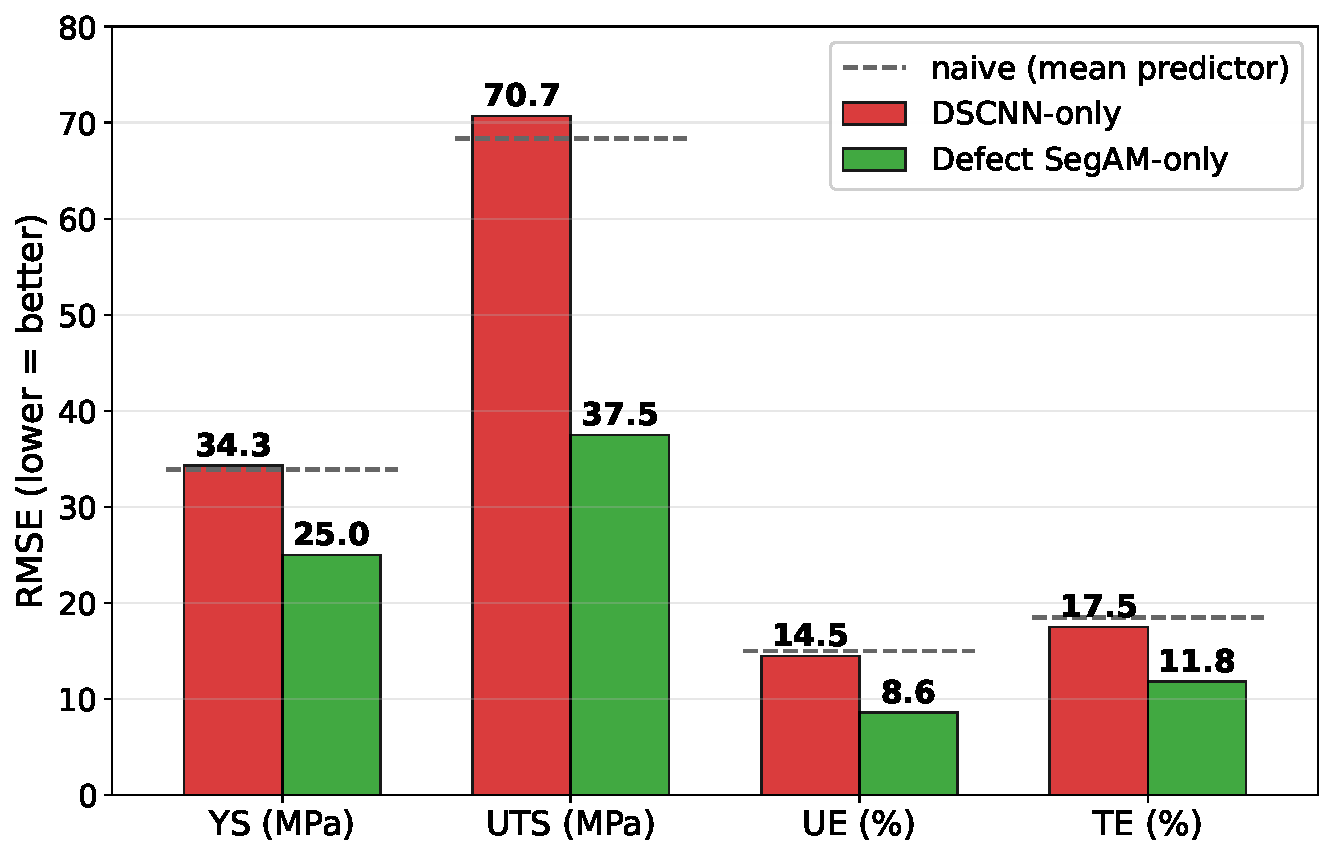
\includegraphics[width=\linewidth]{Figs/Graph_Seg_Compare_DSCNN_vs_DefectSegAM.pdf}
\caption{5-fold 시편 단위 교차검증에서 네 가지 인장 특성(YS, UTS, UE,
TE)에 대한 segmentation-only 물성 예측기의 시편 수준 RMSE. 막대는 DSCNN
기반 변형과 DefectSegAM 기반 변형을 비교하며, 점선은 naive 전역 평균
예측기를 표시한다. DSCNN 기반 변형은 naive 기준선을 개선하지 못하는
반면(YS 와 UTS 에서는 오히려 더 나쁨), DefectSegAM 기반 변형은 일관되게
그리고 큰 폭으로 기준선을 밑돈다. 수치 값은 표~\ref{tab:downstream}에
제시하였다.}
\label{fig:downstream}
\end{figure}

집계·모델·분할·정규화를 동일하게 유지한 채 세그멘테이션 소스만
DefectSegAM 으로 교체하면 결함 신호가 복원된다. DefectSegAM 기반 변형은
$25.0 \pm 1.0$\,MPa (YS), $37.5 \pm 1.2$\,MPa (UTS), $8.6 \pm 0.3$\,\%
(UE), $11.8 \pm 0.3$\,\% (TE) 의 RMSE 를 달성하며, 이는 naive 기준선 대비
각각 26.1\,\%, 45.2\,\%, 42.4\,\%, 36.3\,\% 의 감소이다. 다섯 개 UTS fold
의 RMSE 는 35.7--39.0\,MPa 의 좁은 범위에 분포한다. 참고로,
segmentation-only UTS 수치 37.5\,MPa 는 원 VPPM 논문에서 보고된 DSCNN 단독
결과(40.6\,MPa)~\cite{VPPM_Baseline}와 비견되며---실제로는 3.1\,MPa 더
낮고---센서·형상·스캔 경로 피처를 추가로 사용하는 본 연구의 21-피처
베이스라인 재현 결과(42.9\,MPa)보다도 낮다. 여기서 두 가지 결론이 따른다.
첫째, 이 데이터셋에서 segmentation-only VPPM 변형의 실패는 정적 8차원 집계
표현 자체의 본질적 한계가 아니라, 물성 관련 결함 정보를 너무 적게 담고
있는 세그멘테이션 소스의 결과이다. 둘째, 모든 변형이 동일한 시편 단위
교차검증 분할을 공유하므로, 이 대비는 세그멘테이션 품질에 대한 통제된,
teacher 독립적인 측정이 된다. 즉, DefectSegAM 은 데이터셋 제공 맵이
전달하지 못하는 물성 관련 결함 신호를 복원한다. 절대적인 RMSE 값은
leave-one-build-out 프로토콜에서는 달라질 수 있으나, 이
붕괴-복원(collapse-to-recovery) 대비는 다운스트림 물성 예측 파이프라인에서
DefectSegAM 을 세그멘테이션 소스로 채택하는 직접적인 실험적 근거가 된다.

% -------------------------------------------------------------------------
\subsection{계산 효율}
\label{sec:results-efficiency}

표~\ref{tab:efficiency}는 DefectSegAM 의 계산 비용을 프로파일링한 것으로,
배포 구성(ViT-B/14)과 이전 세대에서 사용한 ViT-S/14 변형의 frozen 및
학습 가능 파라미터 수를 보고한다(구성과 파라미터 분해는
\ref{sec:method-arch}절, 학습 하드웨어와 단계별 소요 시간은
\ref{sec:setup-impl}절). 학습은 GPU 당 배치 크기 4에서 GPU 당 약
20\,GB 의 메모리를 점유하는 것으로 측정되었다. 레이어당 추론
지연시간(latency)과 처리량(throughput)은 아직 벤치마크하지 않았다.
\TODO{DefectSegAM(8-way test-time augmentation 유무 각각)과 재구현 DSCNN
에 대해 동일한 하드웨어에서 단일 레이어 추론 지연시간과 초당 레이어
처리량을 측정하고, 표~\ref{tab:efficiency}의 해당 셀을 채울 것; 재구현
DSCNN 의 파라미터 수를 보고할 것.}

\begin{table}[t]
\centering
\caption{계산 비용 프로파일. 파라미터 수는 DefectSegAM 구성(frozen 인코더
/ 학습 가능 decoder 및 head)에 대해 정확한 값이며, 동일한 하드웨어에서의
추론 시간 측정은 미완료 상태이다. \TODO{지연시간·처리량 열을 기입할 것;
재구현 DSCNN 의 파라미터 수를 추가할 것.}}
\label{tab:efficiency}
\footnotesize
\begin{tabularx}{\textwidth}{@{}>{\raggedright\arraybackslash}Xcccc@{}}
\toprule
모델 & \makecell{Frozen\\파라미터} & \makecell{Trainable\\파라미터} & \makecell{입력 크기\\(px)} & \makecell{레이어당\\지연시간 (ms)} \\
\midrule
DefectSegAM (ViT-B/14, 배포 구성) & 86\,M & 14.6\,M & $1036 \times 1036$ & --- \\
DefectSegAM (ViT-S/14 변형)       & 22\,M & 13.4\,M & $1036 \times 1036$ & --- \\
DSCNN (재구현)~\cite{Scime2020DSCNN} & --- & --- & --- & --- \\
\bottomrule
\end{tabularx}
\end{table}

% -------------------------------------------------------------------------
\subsection{계획된 평가: held-out 사람 GT 비교, cross-machine 일반화,
ablation}
\label{sec:results-planned}

본 소절의 세 가지 평가---사람이 주석한 ground truth 상에서 재구현
DSCNN 과 비교하는 held-out 평가(\ref{sec:results-heldout}절),
cross-machine 일반화 연구(\ref{sec:results-crossmachine}절), 그리고 구성
요소 ablation(\ref{sec:results-ablation}절)---은 \ref{sec:setup}절에서
정의한 프로토콜을 따르지만 아직 수행되지 않았다. 이들에 대해서는 완전한
실험 스캐폴딩(scaffolding)을 제시하고 모든 정량 셀을 미기입(pending)
상태로 표시하며, 각 표는 결과가 확보되는 대로 채운다.

\subsubsection{사람 ground truth 상에서 재구현 DSCNN 과의 held-out 비교}
\label{sec:results-heldout}

본 연구의 핵심 정량적 주장은 DefectSegAM 의 학습 과정에서 어떠한 형태로도
사용된 적이 없는, 사람이 주석한 ground truth 상에서 확립할 예정이다. 평가
세트는 \ref{sec:setup-heldout-peregrine}절의 2025 Peregrine held-out
세트~\cite{Peregrine_v2025_TODO}이며, 베이스라인은
\ref{sec:setup-baselines}절의 재구현 DSCNN~\cite{Scime2020DSCNN}과 선택적
표준 베이스라인(U-Net, DeepLabV3+)의 설정을 따른다.
표~\ref{tab:heldout-main}은 결과 스캐폴드(scaffold)를 제시한다.
\TODO{held-out 평가를 수행할 것: (i) 2025 Peregrine 주석의 라벨 온톨로지가
12-class ORNL 공간과 호환되는지 검증하고 매핑을 문서화할 것; (ii) 원 논문에서
DSCNN 하이퍼파라미터를 옮겨 적어 동일한 코퍼스로 재구현 모델을 학습할 것;
(iii) 표~\ref{tab:heldout-main}의 모든 셀을 공정 기술별 mIoU 와 픽셀
정확도로 채울 것.}

\begin{table}[t]
\centering
\caption{본 연구의 어떤 학습에도 쓰이지 않은 2025 Peregrine held-out
세트(\ref{sec:setup-heldout-peregrine}절)에서의 세그멘테이션 성능. 모든
모델은 \ref{sec:setup-corpora}절의 동일한 코퍼스로 학습한다. mIoU 는
support 가 0이 아닌 클래스들에 대한 mean intersection-over-union 이며,
L-PBF 와 BJ 는 각각 Concept Laser M2 부분집합과 ExOne Innovent 부분집합을
나타낸다. 모든 항목은
미기입(pending) 상태이다. \TODO{held-out 평가 수행 후 기입할 것; 2025 주석의
12-class 공간으로의 라벨 온톨로지 매핑을 확인할 것.}}
\label{tab:heldout-main}
\footnotesize
\begin{tabular}{lcccc}
\toprule
모델 & \makecell{mIoU\\(L-PBF)} & \makecell{mIoU\\(BJ)} & \makecell{mIoU\\(all)} & \makecell{Pixel acc.\\(all)} \\
\midrule
DSCNN (재구현)~\cite{Scime2020DSCNN} & --- & --- & --- & --- \\
U-Net~\cite{Ronneberger2015UNet}            & --- & --- & --- & --- \\
DeepLabV3+~\cite{Chen2018DeepLabV3Plus}     & --- & --- & --- & --- \\
DefectSegAM (제안 모델)                     & --- & --- & --- & --- \\
\bottomrule
\end{tabular}
\end{table}

\subsubsection{Cross-machine 일반화}
\label{sec:results-crossmachine}

동결(frozen)된 파운데이션 모델 피처 위에 DefectSegAM 을 구축한 핵심 동기는
장비·소재·카메라 구성을 가로지르는 전이(transfer)이다. 이 주장을 ORNL
생태계 밖에서 검증하기 위해, 어떠한 장비별 재학습도 없이 모든 학습 소스에
부재한 장비들의 분말 도포(recoating) 이미지에 대해 모델을 평가한다. 평가
세트는 \ref{sec:setup-heldout-crossmachine}절의 저자 수집 cross-machine
세트(Veltz M160/M280 및 EOS 장비)의 정의를 따르며, 2025 Peregrine 세트는
같은 절에서 밝힌 이유로 포함하지 않는다.
표~\ref{tab:crossmachine}은 스캐폴드를 제시하며, 모든 셀에서 재구현
DSCNN 이 비교 모델로 사용된다. \TODO{Veltz M160/M280 및 EOS 이미지를
수집하고 픽셀 라벨링할 것(레이어 수, 소재, 카메라 사양, 라벨링 프로토콜
문서화 예정); 세 개 장비 부분집합 모두에서 두 모델을 실행하고
표~\ref{tab:crossmachine}을 채울 것.}

\begin{table}[t]
\centering
\caption{학습 중 보지 못한 장비에 대한 cross-machine 일반화. 각 행은
held-out 사람 주석 recoating 이미지의 한 장비 부분집합이며, 두 모델 모두
장비별 재학습을 받지 않는다. $\Delta$mIoU 는 DefectSegAM 에서 DSCNN 을 뺀
값이다. 모든 항목은 미기입(pending) 상태이다. \TODO{cross-machine 데이터
수집 및 평가 후 기입할 것; 부분집합별 레이어 수, 소재, 카메라 사양을
문서화할 것.}}
\label{tab:crossmachine}
\footnotesize
\begin{tabularx}{\textwidth}{@{}>{\raggedright\arraybackslash}Xlccc@{}}
\toprule
장비 & 공정 & \makecell{DSCNN\\mIoU} & \makecell{DefectSegAM\\mIoU} & $\Delta$mIoU \\
\midrule
Veltz M160                        & PBF        & --- & --- & --- \\
Veltz M280                        & PBF        & --- & --- & --- \\
EOS 장비 \TODO{모델명}            & PBF        & --- & --- & --- \\
\bottomrule
\end{tabularx}
\end{table}

\subsubsection{Ablation 연구}
\label{sec:results-ablation}

DefectSegAM 의 아키텍처와 학습 레시피에는 여섯 가지 설계 결정이 포함되어
있으며, 각각의 개별 기여는 \ref{sec:results-heldout}절과 동일한 held-out
사람 ground truth 상에서 분리하여 확인할 예정이다:
(i)~이중 이미지 입력 --- 용융 직후(melt) 이미지 $I_0$ 만 또는 분말
도포(powder) 이미지 $I_1$ 만 입력하여 ablation; (ii)~명시적 변화
단서(change cue) --- 식~\eqref{eq:forward}의 융합에서
$\mathbf{F}^{(1)}_s-\mathbf{F}^{(0)}_s$ 차분 항을 제거하여 두 피처 맵의
concatenation 만 남김; (iii)~Stage-1 의사 라벨(pseudo-label) 사전학습 ---
무작위 초기화된 decoder 를 전문가 주석에 직접 미세조정하여 ablation;
(iv)~class-aware 레이어 샘플링 --- 균일 샘플링으로 대체;
(v)~Copy-Paste 증강~\cite{Ghiasi2021CopyPaste} --- 증강 체인에서 제거;
그리고 (vi)~백본 용량 --- ViT-B/14 인코더를 이전 모델 세대에서 사용한
ViT-S/14 인코더로 교체. 여기에 더해 학습
없이 추론 시에만 적용되는 두 가지 옵션, 즉 (vii)~8-way test-time
augmentation 과 (viii)~\ref{sec:method-inference}절의 두 가지 휴리스틱
후처리 규칙의 효과를 같은 held-out 세트에서 정량화한다.
표~\ref{tab:ablation}은 스캐폴드를 제시한다. \TODO{ablation 대상 구성
요소를 제외하고는 동일한 2-stage 레시피로 일곱 가지 구성을 학습하고,
전체 모델에 TTA 와 후처리를 각각 추가한 두 가지 추론 시 옵션과 함께
held-out 사람 GT mIoU 로 표~\ref{tab:ablation}을 채울 것.}

\begin{table}[t]
\centering
\caption{표~\ref{tab:heldout-main}의 held-out 사람 주석 테스트 세트에서
평가한 DefectSegAM 의 구성 요소 ablation. 각 학습 변형은 전체 모델 대비
정확히 하나의 구성 요소만 변경하며, 추론 시 옵션 행은 전체 모델의 학습된
가중치를 그대로 두고 test-time augmentation(TTA) 또는 후처리 규칙만
추가한 것이다. $\Delta$mIoU 는 첫 번째 행 대비 변화량이다. 모든 항목은
미기입(pending) 상태이다. \TODO{ablation 실행 후 기입할 것.}}
\label{tab:ablation}
\footnotesize
\begin{tabular}{lcc}
\toprule
구성 & mIoU & $\Delta$mIoU \\
\midrule
DefectSegAM (전체 모델, 단일 forward)        & --- & ---  \\
\midrule
\multicolumn{3}{@{}l}{\emph{학습 변형}}\\
단일 이미지: 용융 직후 $I_0$ 만              & --- & --- \\
단일 이미지: 도포 직후 $I_1$ 만              & --- & --- \\
차분 항 $\mathbf{F}^{(1)}_s-\mathbf{F}^{(0)}_s$ 제거 & --- & --- \\
Stage-1 pseudo-label 사전학습 제거           & --- & --- \\
Class-aware 샘플링 제거                      & --- & --- \\
Copy-Paste 증강 제거                         & --- & --- \\
ViT-S/14 백본 (22\,M frozen)                 & --- & --- \\
\midrule
\multicolumn{3}{@{}l}{\emph{추론 시 옵션 (전체 모델)}}\\
$+$ 8-way TTA                                & --- & --- \\
$+$ 8-way TTA $+$ 후처리 규칙 1--2           & --- & --- \\
\bottomrule
\end{tabular}
\end{table}
